\documentclass{article}

\usepackage[margin=1in]{geometry}
\usepackage{fancyhdr}
\usepackage{amsmath}
\usepackage{amssymb}
\usepackage{listings}
\usepackage{graphicx}
\usepackage{enumerate}
\usepackage{tikz}
\usetikzlibrary{automata,positioning}


\pagestyle{fancy}

\lhead{CS 373 - Section @ 12AM\\ Homework 1}
\rhead{Drew Cross (ddcross2) \\
      \emph{Partners:} Bryan Plummer, Eric Parsons}
\lfoot{}
\cfoot{}
\rfoot{}

\begin{document}


\section*{Homework 1}

\subsection*{Problem 1}
\begin{enumerate}[a)]
\item $\{w\ |\ w$ does not contain three consecutive 1's and does not start with 00 \}

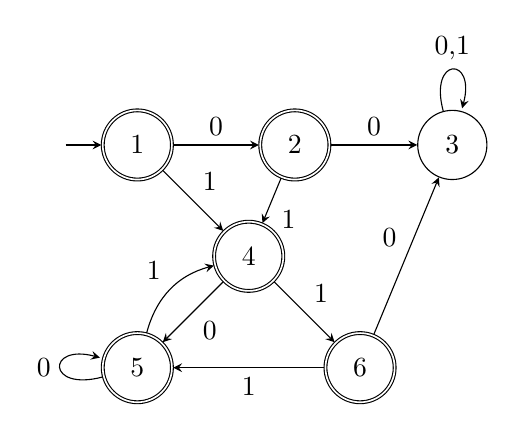
\begin{tikzpicture}[%
    >=stealth,
    node distance=2cm,
    on grid,
    auto
    ]
    \node[initial,initial text=,state,accepting] (1)       {1};
    \node[state, accepting] (2) [right of=1] {2};
    \node[state] (3) [right of=2] {3};
    \node[state, accepting] (4) [below right of=1] {4};
    \node[state, accepting] (5) [below left of=4] {5};
    \node[state, accepting] (6) [below right of=4] {6};

    \path[->] (1) edge node {0} (2);
    \path[->] (1) edge node {1} (4);
    \path[->] (2) edge node {0} (3);
    \path[->] (2) edge node {1} (4);
    \path[->] (3) edge[loop above] node {0,1} (3);
    \path[->] (4) edge node {0} (5);
    \path[->] (4) edge node {1} (6);
    \path[->] (5) edge[loop left] node {0} (5);
    \path[->] (5) edge[bend left] node {1} (4);
    \path[->] (6) edge node {0} (3);
    \path[->] (6) edge node {1} (5);

    \end{tikzpicture}

    \item \{$w$ $|$ the total number of 0's in $w$ congruent to 2 modulo 3 and the total number
    of 1's in $w$ is congruent to 4 modulo 5\}

    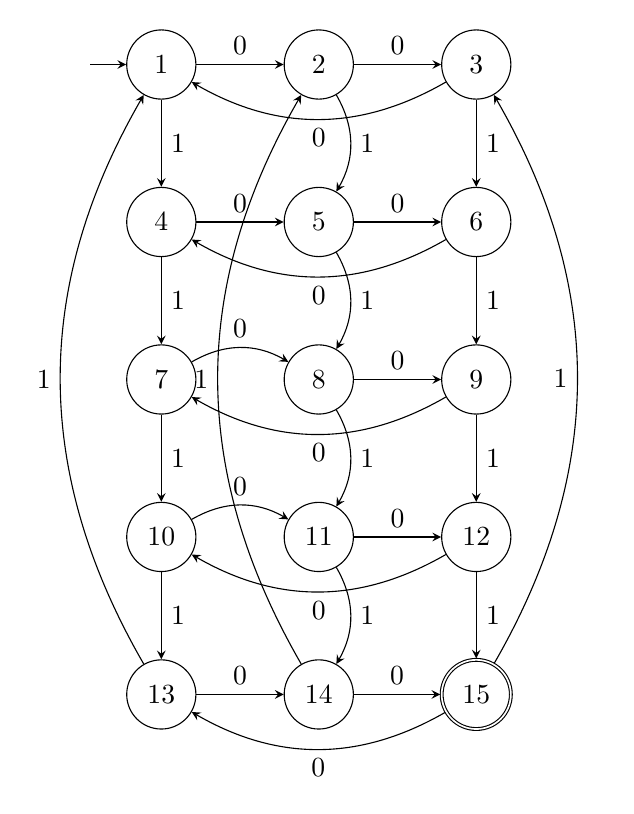
\begin{tikzpicture}[%
        >=stealth,
        node distance=2cm,
        on grid,
        auto
        ]
        \node[initial, initial text=,state] (1)  {1};
        \node[state] (2) [right of=1] {2};
        \node[state] (3) [right of=2] {3};
        \node[state] (4) [below of=1] {4};
        \node[state] (5) [right of=4] {5};
        \node[state] (6) [right of=5] {6};
        \node[state] (7) [below of=4] {7};
        \node[state] (8) [right of=7] {8};
        \node[state] (9) [right of=8] {9};
        \node[state] (10) [below of=7] {10};
        \node[state] (11) [right of=10] {11};
        \node[state] (12) [right of=11] {12};
        \node[state] (13) [below of=10] {13};
        \node[state] (14) [right of=13] {14};
        \node[state, accepting] (15) [right of=14] {15};

        \path[->] (1) edge node {0} (2);
        \path[->] (2) edge node {0} (3);
        \path[->] (4) edge node {0} (5);
        \path[->] (5) edge node {0} (6);
        \path[->] (7) edge[bend left] node {0} (8);
        \path[->] (8) edge node {0} (9);
        \path[->] (10) edge[bend left] node {0} (11);
        \path[->] (11) edge node {0} (12);
        \path[->] (13) edge node {0} (14);
        \path[->] (14) edge node {0} (15);
        %Loop-backs:
        \path[->] (3) edge[bend left] node {0} (1);
        \path[->] (6) edge[bend left] node {0} (4);
        \path[->] (9) edge[bend left] node {0} (7);
        \path[->] (12) edge[bend left] node {0} (10);
        \path[->] (15) edge[bend left] node {0} (13);

        % 1 lines
        \path[->] (1) edge node {1} (4);
        \path[->] (4) edge node {1} (7);
        \path[->] (7) edge node {1} (10);
        \path[->] (10) edge node {1} (13);

        \path[->] (2) edge[bend left] node {1} (5);
        \path[->] (5) edge[bend left] node {1} (8);
        \path[->] (8) edge[bend left] node {1} (11);
        \path[->] (11) edge[bend left] node {1} (14);

        \path[->] (3) edge node {1} (6);
        \path[->] (6) edge node {1} (9);
        \path[->] (9) edge node {1} (12);
        \path[->] (12) edge node {1} (15);

        % Loop-backs
        \path[->] (13) edge[bend left] node {1} (1);
        \path[->] (14) edge[bend left] node {1} (2);
        \path[->] (15) edge[bend right] node {1} (3);


    \end{tikzpicture}
    \item $\Sigma^{*}\setminus((\Sigma\Sigma\Sigma)^{*}\cup(\Sigma\Sigma)^{*}\cup\emptyset^{*})$

    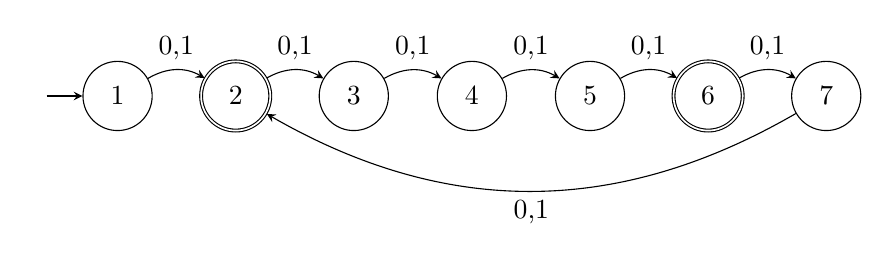
\begin{tikzpicture}[%
        >=stealth,
        node distance=1.5cm,
        on grid,
        auto
        ]
        \node[initial, initial text=,state] (1)  {1};
        \node[state, accepting] (2) [right of=1] {2};
        \node[state] (3) [right of=2] {3};
        \node[state] (4) [right of=3] {4};
        \node[state] (5) [right of=4] {5};
        \node[state, accepting] (6) [right of=5] {6};
        \node[state] (7) [right of=6] {7};

        \path[->] (1) edge[bend left] node {0,1} (2);
        \path[->] (2) edge[bend left] node {0,1} (3);
        \path[->] (3) edge[bend left] node {0,1} (4);
        \path[->] (4) edge[bend left] node {0,1} (5);
        \path[->] (5) edge[bend left] node {0,1} (6);
        \path[->] (6) edge[bend left] node {0,1} (7);
        \path[->] (7) edge[bend left] node {0,1} (2);

    \end{tikzpicture}
\end{enumerate}

\newpage

\subsection*{Problem 2}
\begin{enumerate}[a)]

    \item NFA to DFA

        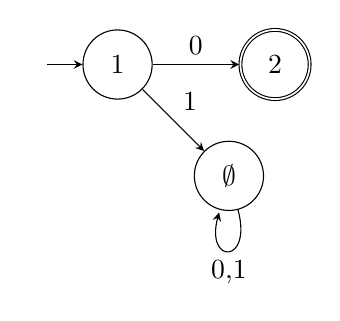
\begin{tikzpicture}[%
            >=stealth,
            node distance=2cm,
            on grid,
            auto
            ]
            \node[initial, initial text=,state] (1)  {1};
            \node[state, accepting] (2) [right of=1] {2};
            \node[state] (3) [below right of=1] {$\emptyset$};

            \path[->] (1) edge node {1} (3);
            \path[->] (3) edge[loop below] node {0,1} (3);
            \path[->] (1) edge node {0} (2);

        \end{tikzpicture}
    \item NFA to DFA

        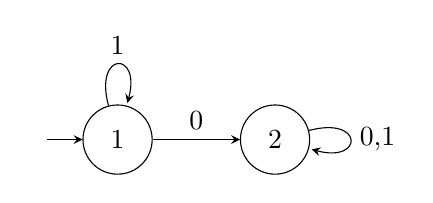
\begin{tikzpicture}[%
            >=stealth,
            node distance=2cm,
            on grid,
            auto
            ]
            \node[initial, initial text=, state] (1) {1};
            \node[state] (2) [right of=1] {2};

            \path[->] (1) edge[loop above] node {1} (1);
            \path[->] (1) edge node {0} (2);
            \path[->] (2) edge[loop right] node {0,1} (2);
        \end{tikzpicture}
\end{enumerate}

\newpage

\subsection*{Problem 3}
To prove that an operation is closed under regular languages we need to construct a DFA, NFA
or give a regular expression that accepts the new language the function defines. \\

\begin{enumerate}[a)]
    \item $f(L)=\{x:xy \in L \text{ for some } y\in\Sigma^*\}$ \\
    Abstract: Take all the states that are reached in route to an accept state and make them 
    accept states. \\

    Let $N_1 = (Q_1, \Sigma, \delta_1, q_1, F_1)$ recognize $xy$ \\
    Construct $N$ to recognize $f(L)$ as follows:\\
    $N = (Q, \Sigma, \delta, q_0, F)$ \\
    $Q = Q_1$ \\
    $\Sigma = \Sigma$ \\
    $q_0 = q_1$ \\
    $\delta = \delta_1$ \\
    $F = \{r\ |\ r_1r_1\ ...\ r_n$ where $r_n $ is the sequence of states to get to an accept 
            state in  $N_1\}$
    \[ \square \]

    \item $r(L)=\{x^R:x\in L\}$ \\
    Abstract: Reverse all transition lines between states. Make a new state with $\epsilon$
    transitions to all current accept states. Take all accept states in the machine and
    make them regular, non-accept states. Then take the start state and make it an accept state
    and finally make the newly included state the start state.\\

    Let $N_1 = (Q_1, \Sigma, \delta_1, q_1, F_1) $ \\
    Now construct $N$ to recognize $r(L)$ as follows:\\
    $N = (Q, \Sigma, \delta, q_0, F) $ \\
    $Q = Q_1 \cup \{ q_0\}$ where $q_0 \notin Q_1$ \\
    $\Sigma = \Sigma$ \\
    $q_0 = q_1$ \\
    $\delta$ is given by \\
    $\delta(q,a) = $
    $\left\{
        \begin{array}{lr}
            F_1 & $ if $ q_0 = q_1 $ and $ a = \epsilon \\
            \{q \in Q_1 | \delta(q,a) = q_1\} & $ if $ q_1 \in Q_1 \\
            \emptyset & $otherwise$
        \end{array}
    \right. $\\
    $F = \{q_0\}$ \\
    \[ \square \]

    \item $Q(L_1,L_2)=\{w:wx \in L_1 \text{ and } x\in L_2\}$

    Abstract: We now need to construct a new machine $N = (Q, \Sigma, \delta, q_0, F) $
    that accepts
    the sequence of symbols in $M_1$ but not $M_2$. $M_1$ contains $M_2$
    so we can make a machine by identifying the states that transition from $M_1$ to $M_2$
    and make those states accept states. Then we need to make all accept states in $M_2$
    normal states.


    Formally:
    Let $M_1 = (Q_1, \Sigma_1, \delta_1, q_1, F_1)$ recognize $L_1$ or $L(M_1) = L_1$ 
    and $M_2 = (Q_2, \Sigma_2, \delta_2, q_2, F_2)$ recognize or $L(M_2) = M_2$. \\

    $N = (Q, \Sigma, \delta, q_0, F) $\\
    $Q = Q_1 $\\
    $\Sigma = \Sigma$ \\
    $q_0 = q_1$ \\
    $\delta = \delta_1$ \\
    $F = \{q_1\ |\ q_2 = \delta_1(q_1,a)$ where $q_2 \in Q_2 $ and $q_1 \in Q_1\} 
    \cup \{ F_1 \cap \overline{F_2} \}$
    \[ \square \]
\end{enumerate}

\newpage

\subsection*{Problem 4}

\begin{enumerate}[a)]
\item FST

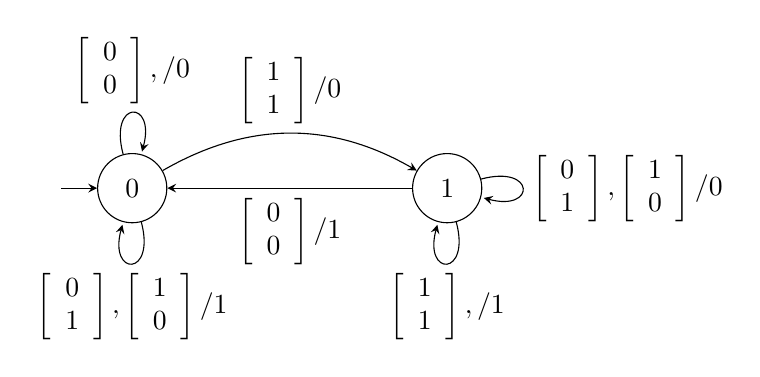
\begin{tikzpicture}[%
    >=stealth,
    node distance=4cm,
    on grid,
    auto
    ]
    \node[initial,initial text=,state] (0)       {0};
    \node[state] (1) [right of=0] {1};

    \path[->] (1) edge node {$\left[
                            \begin{array}{l} 0 \\ 0 \end{array}\right]
                            /1$} (0);
    \path[->] (0) edge[bend left] node {$\left[
                            \begin{array}{l} 1 \\ 1 \end{array}\right]/0$} (1);


    \path[->] (1) edge[loop right] node {$
    \left[\begin{array}{l} 0 \\ 1 \end{array}\right],
    \left[\begin{array}{l} 1 \\ 0 \end{array}\right]
                            /0$} (1);

    \path[->] (1) edge[loop below] node {$
    \left[\begin{array}{l} 1 \\ 1 \end{array}\right],
                            /1$} (1);

    \path[->] (0) edge[loop below] node {$
    \left[\begin{array}{l} 0 \\ 1 \end{array}\right],
    \left[\begin{array}{l} 1 \\ 0 \end{array}\right]
                            /1$} (0);

    \path[->] (0) edge[loop above] node {$
    \left[\begin{array}{l} 0 \\ 0 \end{array}\right],
                            /0$} (0);

\end{tikzpicture}
    \item Let $\Sigma_1=\{a,b\}$ and $Q_n=\{q_1,q_2,...,q_n\}$ be sets.
    
    Let $\mathbb{D}_n=\{D_n\;|\;D_n=(Q_n,\Sigma_1,d:Q_n\times\Sigma_1\rightarrow Q_n,q_0\in Q_n,F\subseteq Q_n)\}$ be the set of all DFAs with $n$ states.
    
    \begin{enumerate}[i)]
        \item Create an encoding for $\mathbb{D}_n$ using the symbols from $\Sigma_2=Q_n \cup \{\$\}$ (here, $\$$ is just one additional symbol you can use.)  In other words, create a one-to-one function $M: \mathbb{D}_n\rightarrow\Sigma_2^{*}$.\\

We need to create a one-to-one functoin $M:\mathbb{D}_n \rightarrow \Sigma^*_2$ \\
We can create an encoding as follows: \\
$<$Start State$>$ $\$<$Transition pairs for the first symbol$>\$$ $<$...$>$ $\$\$<$
list of accept states$>\$$

Thus this DFA would be encoded as follows:\\
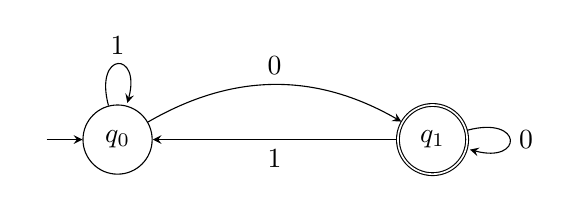
\begin{tikzpicture}[%
    >=stealth,
    node distance=4cm,
    on grid,
    auto
    ]
    \node[initial,initial text=,state] (0)       { $q_0$ };
    \node[state, accepting] (1) [right of = 0] { $q_1$ };

    \path[->] (0) edge[loop above] node {1} (0);
    \path[->] (0) edge[bend left] node {0} (1);
    \path[->] (1) edge[loop right] node {0} (1);
    \path[->] (1) edge node {1} (0);
\end{tikzpicture}\\[5pt]
    $q_0\$q_0q_1q_1q_1\$q_0q_0\$q_1q_0\$\$q_1\$ $ \\
    For $\Sigma = \{ 0,1 \}$
        \item Give a formal description of an FST that takes any encoded $D_n\in\mathbb{D}_n$, concatenated with a string $w\in\Sigma_1^{*}$ and outputs the states visited by $D_n$ when processing $w$.  If the input string does not follow this format, your FST should output the empty string.  The transitions in your FST may have $\varepsilon$ on the input or output.\\

Formal Definitions:
$M:$\\
$Q=\{m_0,m_1,\ ...\ \}$\\
$\Sigma = \Sigma^*_2$ \\
$\Gamma = \{\epsilon\}$ \\
$q_0 = m_0 \in Q$ \\
$\delta = Q \times E \rightarrow (Q \cup \{$ The start states of all N machines $\}) \times \Gamma $ \\

$N:$\\
$Q=\{n_0,n_1,\ ...\ \}$\\
$\Sigma = \Sigma^*_2$ \\
$\Gamma = \{\epsilon\}$ \\
$q_0 = n_0 \in Q$ \\
$\delta = Q \times E \rightarrow (Q \cup \{$ The start states of all P machines $\}) \times \Gamma $ \\

$P:$\\
$Q=\{p_0,p_1,\ ...\ \}$\\
$\Sigma = \Sigma^*_2$ \\
$\Gamma = \{\epsilon\}$ \\
$q_0 = p_0 \in Q$ \\
$\delta = Q \times E \rightarrow (Q \cup \{$ The start states of all R machines $\}) \times \Gamma $ \\

$R:$\\
$Q=\{r_0,r_1,\ ...\ \}$\\
$\Sigma = \Sigma_1$ \\
$\Gamma = \{x | x \in w\}$ \\
$q_0 = r_0 \in Q$ \\
$\delta = Q \times E \rightarrow Q \times \Gamma $


    \end{enumerate}
\end{enumerate}

\newpage

\subsection*{Problem 5}

\begin{enumerate}[a)]
\item

In order to prove that the set of all DFAs containing no unreachable states that use
an input alphabet $\Sigma$ and accept $A$ is countably infinite we need to show that there
is a bijection between the natural numbers and the set of all DFAs.\\[5pt]
Let $n = |Q|$ for some DFA $M$ \\
There is a finite number of ways we can arrange the transitions between all the states
$q \in Q$\\
There is also a finite number of transitions, $\delta$, $n^{|\Sigma|n}$.\\
Each state needs $|\Sigma|$ outward transitions and each transition points to one $q$.\\
The start state is also finite: $q_0 \in Q$. \\
There are $2^n$ permutations of the set $F$, in other words, there are $2^n$ different ways
we can rearrange the accept and non-accepting states.\\
So for each $n$ we have a finite set of configurations of DFAs.\\
Now we can map the natural numbers to $n$ - the set of possible configurations of DFAs with
$|Q| = n$.\\

Sets: $\{$DFAs for $n=0\},\ \{$DFAs for $ n=1\},\ ...\ ,\{$DFAs for $ n=i-1\}$\\
Where $i \in \mathbb{N}$

Because the set of DFAs for a given $|Q|$ is finite, we can map the natural numbers to the
sets by using $|Q|$ Therefore this set is countably infinite since we have successfully
mapped the natural numbers to the set of all DFAs representing a regular language.
\[\square\]


\end{enumerate}

\newpage

\subsection*{Problem 6}

\begin{enumerate}[a)]
    \item Prove that $L^*L^*=L^*$ for any language L.\\
    By the definition of the Kleene Star:\\
    Let $L_1^* = \{x_1x_2\ ...\ x_k | k \geq $ and $ x_i \in L_1 \}$ and \\
    Let $L_2^* = \{y_1y_2\ ...\ y_m | m \geq $ and $ y_i \in L_2 \}$ \\[5pt]
    Therefore: \\
    $L_1^*L_2^* = \{ xy\ |\ x \in L_1 $ and $ y \in L_2 \}$ \\
    So $L_1^*L_2^*$ has the form: \\
    $\{x_1x_2 \ ...\ x_ky_1y_2\ ...\ y_m $ for $m,k \geq 0$ and $x_i \in L_1$ and $y_i \in L_2\}$

    But $L_1 = L_2$ \\
    So we can write this as: \\
    $L^*L^* = \{x_1x_2\ ... x_kx_{k+1}x_{k+2}\ ...\ x_m$ for $m,k \geq 0 $ and $ x_i \in L \}$

    Which has the same form as the definition of the Kleene Star:\\
    $L^* = \{x_1x_2\ ...\ x_m$ for $ m \geq 0 $ and $ x_i \in L\}$\\
    \[ \square\]

    \item Prove that $L^{**}=L^*$ for any language L.\\
    $L^* = \{ x_1x_2\ ...\ x_k$ for some $ k \geq 0 \}$\\
    Let $y \in L^*$ That is: $y = (x_1x_2\ ...\ x_k)$\\
    So: \\
    $L^{**} = \{(x_1x_2\ ...\ x_k)_0(y_1y_2\ ...\ y_k)_1 \ ...\ (z_1z_2\ ...\ z_k)_n\ |\ 
    n,k \geq 0 $ and $ x_i,y_i,\ ...\ z_i \in L \}$\\
    Which has the same form as the definition of the Kleene Star: \\
    $L^* = \{x_1x_2\ ...\ |\ k \geq 0$ and $ x_i \in L\}$
    \[ \square \]
    \item Given a unary alphabet (e.g. $\Sigma = {1}$) write an equation for
    $|\Sigma^* \backslash ((\Sigma^n)^*(\Sigma^{n+1})^*)|$ in terms of $n$. Explain your answer.\\
    $\Sigma^*=$ All strings with zero or more symbols.\\
    $(\Sigma^n)^* =$ All strings that are zero or a multiple of length n. \\[5pt]

    If $n=0\ |\Sigma^* \backslash ((\Sigma^n)^*(\Sigma^{n+1})^*)| = 0$ \\
    If $n=1\ |\ ...\ | = 0 $ \\
    If $n=2\ |\ ...\ | = 1 $ \\
    If $n=3\ |\ ...\ | = 3 $ \\
    If $n=4\ |\ ...\ | = 6 $ \\
    If $n=5\ |\ ...\ | = 10 $ \\

    By inspection we can see that the sequence follows: $\sum_{i=0}^n{i-1}$ \\[5pt]
    $\sum_{i=0}^n{i-1} = \sum{i} - \sum{1}$ \\[5pt]
    And these two summations have known closed forms: \\[5pt]
    $\frac{n(n+1)}{2}$ and $n$ respectivly.\\[5pt]
    So:
    $\frac{n(n+1)}{2} - n$\\
    $=\frac{n(n-1)}{2} $\\


    \end{enumerate}

    \end{document}
